\documentclass[11pt,a4paper]{article}

\usepackage{amsmath}
\usepackage{amsfonts}
\usepackage{amssymb}
\usepackage{graphicx}
\usepackage{xeCJK}
\usepackage{graphicx}
\usepackage{wrapfig}
\setCJKmainfont[BoldFont=思源黑体 Medium,ItalicFont=方正楷体_GBK]{思源宋体}
\setlength{\parindent}{2em}
\newcommand{\nianfen}[1]{\hspace{-2em}{(#1\textbf{·}\textit{青岛})}}
\usepackage[left=2.56cm, right=2.56cm, top=3.18cm, bottom=3.18cm]{geometry}
\begin{document}	
	\nianfen{2017}在如图所示电路中,电流表量程为 0~0.6A,电压表量程为 0~3V,电阻$R_2$的阻值为$20Ω$,灯泡$R_1$的阻值和同一电源的电压均保持不变。\textbf{请画出该题的各个等效电路图。}
	\begin{wrapfigure}{r}{0.3\linewidth}
		\includegraphics[width=\linewidth]{2017.bmp}
	\end{wrapfigure}
	
	(1)只闭合开关$\rm S_2$、$\rm S_3$时,电流表示数为 0.2A,求电源电压是多少.
	
	(2)只闭合开关$\rm S_1$、$\rm S_2$、$\rm S_3$时,$R_1$正常发光,电路总功率为 2.4W,求$R_1$的阻值是多少.
	
	(3)只闭合开关$\rm S_1$,滑动变阻器$R_3$的滑片调至最右端,$R_3$两端的电压为$U_3$;再将电源更换,保持滑片位置不变,$R_3$两端的电压变为$U_3'$,电流表示数为 0.15A。已知$U_3:U_3'$=$2:3$。求更换电源后,只闭合开关$\rm S_1$、$\rm S_4$时,在不损坏电流表、电压表和灯泡的情况下,$R_3$的阻值变化范围是多少?
	\clearpage
	
	\nianfen{2016}如图甲所示电路,电源电压保持不变。小灯泡$ L $标有“4V 1.6W”字样,滑动变阻器R1的最大阻值为20Ω,定值电阻$ R_2=20Ω $,电流表的量程为0~0.6A,电压表的量程为0~3V。\textbf{请画出该题的各个等效电路图}。求:
	
	\begin{wrapfigure}{r}{0.5\linewidth}
		\includegraphics[width=\linewidth]{2016}
	\end{wrapfigure}
	
	(1)小灯泡正常工作时的电阻是多少?
	
	(2)只闭合开关$\rm S $、$\rm S_2 $ 和$\rm S_3 $,移动滑动变阻器$ R_1 $的滑片$ P $使电流表示数为0.5A时,$ R_2 $消耗的电功率为1.25 W。此时滑动变阻器 $ R_1 $接入电路中的阻值是多少?
	
	(3)只闭合开关S和$\rm S_1 $,移动滑动变阻器$ R_1 $的滑片$ P $,小灯泡$ L $的$ I-U $图象如图乙所示。在保证各元件安全工作的情况下,滑动变阻器$ R_1 $允许的取值范围是多少?
	\clearpage
	
	\begin{wrapfigure}{r}{0.3\linewidth}
		\includegraphics[width=\linewidth]{2015}
	\end{wrapfigure}

	\nianfen{2015}如图所示,电源电压和小灯泡的阻值均保持不变。小灯泡$ R_1 $标有“4V 1.6W”字样,$ R_2=20$Ω,滑动变阻器$ R_3 $允许通过的最大电流为1A,电流表的量程为0~0.6A,电压表的量程为0~3V。\textbf{请画出每个小题的等效电路图}。

	(1)只闭合开关$\rm S_2 $,电压表的示数为2V,则$R_2$消耗的电功率是多少?
	
	(2)在不损毁各元件的情况下,若闭合所有开关,滑动变阻器$R_3$消耗的最大电功率和最小电功率之比为$3:1$;若只闭合$\rm S_3$,小灯泡$R_1$消耗的电功率变化范围是多少?
	\clearpage
	
	\begin{wrapfigure}{r}{0.3\textwidth}
	\includegraphics[width=\linewidth]{2014}
	\end{wrapfigure}

	\nianfen{2014}在如图所示的电路中,电源电压和小灯泡的阻值均保持不变,电源电压 $ U=6 $V,小灯泡R2标有"6V  3W"字样,电流表的量程为 0~0.6A,电压表的量程为 0~3V,滑动变阻器 $ R——2 $ 的最大阻值为 20Ω,\textbf{请画出该题的各个等效电路图}.
	
	(1)只闭合开关 $\rm S_1 $ 和 $\rm S_2 $ 时,电路消耗的功率为 6W,则闭合开关 $\rm S_1 $、$\rm S_2 $和$\rm S_3 $时,电路的总
	电阻 $ R $=?
	
	(2)在不损坏各元件的情况下,只闭合开关 $\rm S_1 $ 时,$ R_1 $ 消耗的最大功率为 $ P_1 $,只闭合开关$\rm S_2 $时,R2消耗的最小功率为 $ P_2 $,则 $ P_1:P_2= $?
	\clearpage
	
	\begin{wrapfigure}{r}{0.3\linewidth}
		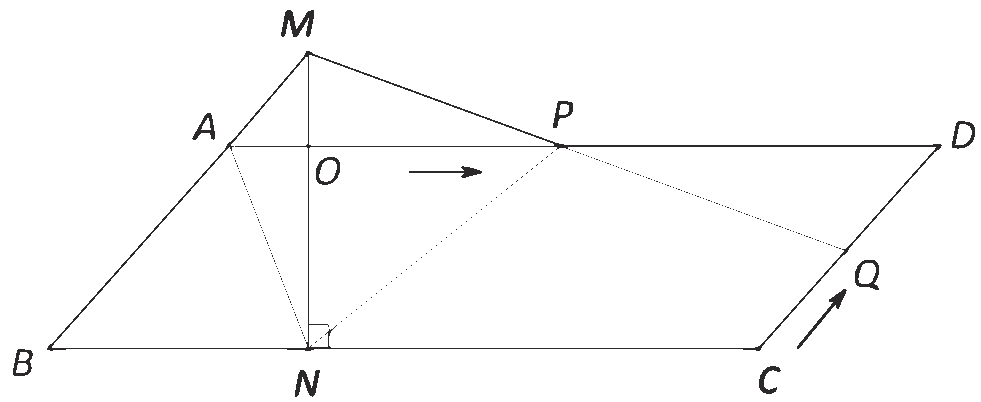
\includegraphics[width=\linewidth]{2013}
	\end{wrapfigure}
	
	\nianfen{2013}在如图所示的电路中,电源电压和各灯泡的阻值均保持不变。电流表的量程为 0~3A,灯泡 $ L_1 $ 的电阻 $ R_1=10 $Ω .请画出该题的各个等效电路图。
	
	(1)只闭合开关 $\rm S_1 $、$\rm S_4 $ 时,电流表的示数为 1A。当将滑动变阻器滑片拨至中点处,再将 $\rm S_2 $闭合时,电流表的示数为 1.5A,则在不损坏电流表的情况下,滑动变阻器可以消耗的最大功率与最小功率之比为多少?
	
	(2)只闭合 $\rm S_3 $ 时,电路消耗的最大功率为$ P_1 $;只闭合 $\rm S_4$、 $\rm S_5 $ 时,电路消耗的最小功率为$ P_2 $;只闭合 $\rm S_2 $、$\rm S_3 $、$\rm S_5 $ 时,电路消耗的最小功率为$ P_3 $。已知 $ P_1:P_2:P_3=42:35:30 $,则 $ R_2 $、$ R_3 $ 的限值各为多少?

\end{document}